% Adriano Bassignana nov 2017
% Program for creating a linear index useful for the construction of a compass on a conical support
% The program can be modified and adapted for the construction of other types of numeric indexes.
% The font used is OCR-B which allows to have alphabetic and numeric symbols very similar
% to those used in analogue flight gauges in the 50s and 80s
% You must have installed OCR-B in OTF format that has a GPL-2 and later compatible license.
% The font is present in the texlive-fonts-extra package
% 
% Explanation:
%
% \documentclass{standalone} is particular class that non have a size, but the size is define from
% the document itself
\documentclass[tikz,margin=0pt]{standalone}
% \usepackage{tikz} is the package that contain the graphics command as \draw etc ...
% The package is describe in this document: https://www.sharelatex.com/learn/TikZ_package
\usepackage{tikz}
% If the graduate dials is for analogical gauges period 50-70 years, this font is ok
% OCR is open-source package deposited in the CTAN repository: https://www.ctan.org/pkg/ocr-b
% Opentype can be used on Linux and Mac machines
% (I do not know if it's possible in Windows, but I think of it),
% you can always download it from the CTAN site at this address:
% https://www.ctan.org/tex-archive/fonts/ocr-b-outline
\usepackage{ocr}
\tikzset{font={\fontsize{12pt}{10}\selectfont}}
% Defines the font size to use, the first number defines the font size,
% the second number the dimensional family from which the font is taken.
% It can be assumed that there are differences between a dimensional family 10 and a 12 dimensional font.
\begin{document}
	% The link OCR package documentation is this: http://ctan.mirror.garr.it/mirrors/CTAN/macros/latex/contrib/ocr-latex/ocr.pdf
	% \ocrfamily - Normal font family
	% \ocrnegfamily - Family negative fonts
	{\ocrfamily
		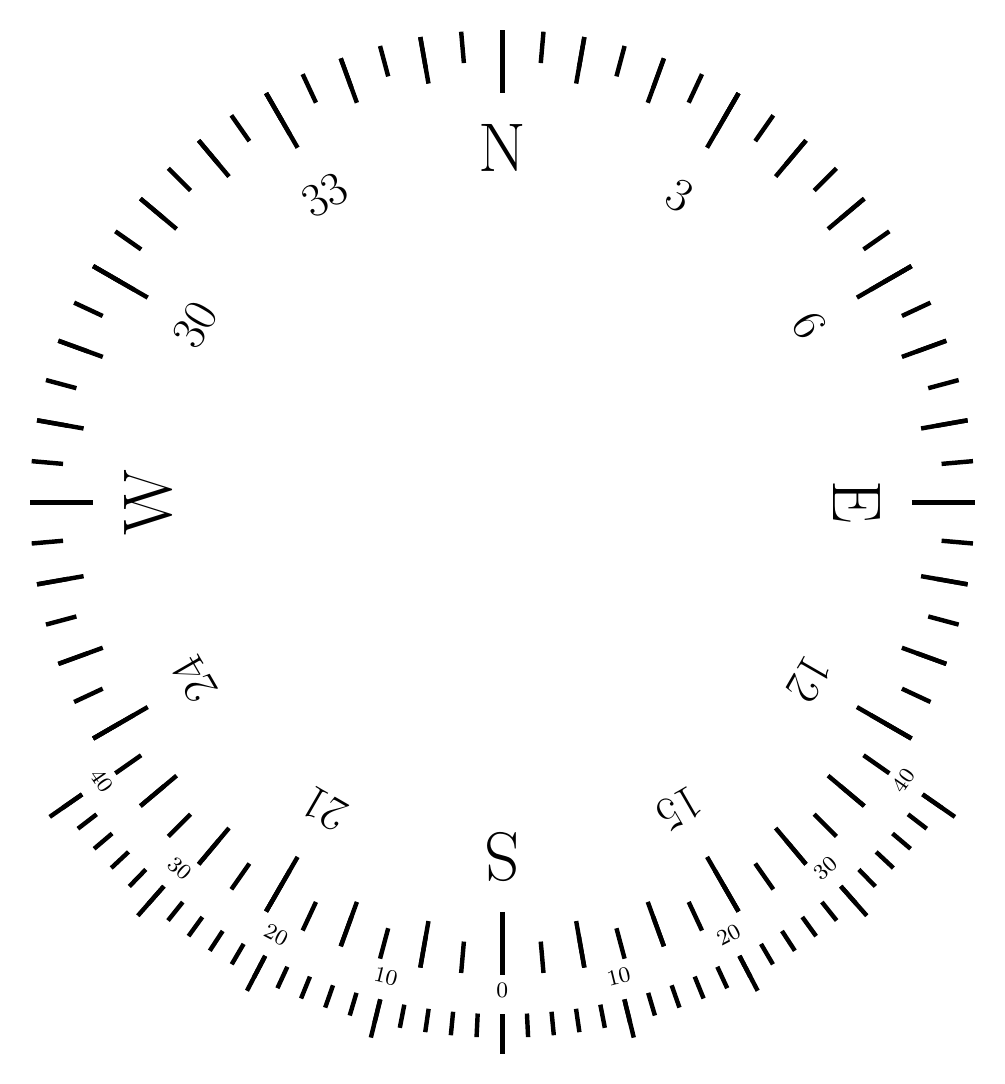
\begin{tikzpicture}
		%1° Rays
		\foreach \a in {0, 5,...,355}
		\draw[ultra thick] (\a:5.6) -- (\a:6);
		%5° Rays
		\foreach \a in {0, 10,...,359}
		\draw[ultra thick] (\a:5.4) -- (\a:6);     
		%10° Rays
		\foreach \a in {0, 30,...,359}
		\draw[ultra thick] (\a:5.2) -- (\a:6);
		%Angle labels 
		\foreach \a in {30, 60, 120, 150, 210, 240, 300, 330}
		\pgfmathtruncatemacro\result{(360 - \a)/10}
		\draw (\a + 90: 4.5) node[rotate=\a] {\LARGE\result};
		% Wind rose labels
		\draw (90: 4.5) node[rotate=0] {\Huge{N}};
		\draw (360: 4.5) node[rotate=270] {\Huge{E}};
		\draw (270: 4.5) node[rotate=180] {\Huge{S}};
		\draw (180: 4.5) node[rotate=90] {\Huge{W}};
		\foreach \b in {-40,-38,...,40}
		\edef\c{-90 - \b * 1.38}
		\draw[ultra thick] (\c:6.5) -- (\c:6.8);
		\foreach \b in {-40,-30,...,40}
		\edef\c{-90 - \b * 1.38}
		\draw[ultra thick] (\c:6.5) -- (\c:7);
		\foreach \b in {-40,-30,...,40}
		\edef\c{-90 - \b * 1.38}
		\pgfmathtruncatemacro\result{abs(\b)}
		\draw (\c:6.2) node[rotate=\c+90] {\footnotesize\result};
		\end{tikzpicture}
	}
\end{document}